\documentclass[a4paper,11pt]{article}
\usepackage[utf8]{inputenc}
\usepackage{minted}
\usepackage{hyperref}
\usepackage{graphicx}
\usepackage{float}


\title{
    \textbf{FSM}
}
\author{Sahidev1}
\date{September 2, 2024}

\begin{document}

\maketitle

\section*{Introduction}
I write this paper/document to deepen my knowledge of Finite State Machines and to have it at hand for the future in case I need a refresher on the topic. Note that the main purpose of this paper is to help understand FSM's, and not to give a strict theoretical description. 

\section*{Finite state machine components}
The components of a Finite state machine are:
\begin{itemize}
    \item Input set I
    \item State set S
    \item $S_0$ is the initial state and $S_0 \in S$
    \item Set of final states F, can be empty
    \item Set of outputs O, can be empty
\end{itemize}


The input set contains all possible inputs that a state can receive. The state set is the set of all states. The initial state is the starting state of the FSM. The set of final states is the set of valid stopping states of the FSM, essentially the states in which the FSM considers its work finished; the final-state set can be empty. The output set contains the set of outputs. The output set can be empty. The most important components to consider are I, S, $S_0$ and F, the output set is primarily relevant in the context of transducers, see below. 


\section*{Finite state machine types}
\subsection*{Deterministic finite automaton}
A Deterministic Finite Automaton(DFA) is predictable. From the current state, each unique input is associated with a single unique next state, thus from the current state you can always predict the next state on different inputs. 

\subsection*{Non-deterministic Finite Automaton}
A Non-deterministic Finite Automaton(NFA) is primarily a theoretical abstraction. An NFA is unpredictable; the current state might transition to multiple other states based on one single unique input. An NFA can also accept empty inputs $\epsilon$. An NFA can also have no next state at all. An NFA can transition to other possible states from a single input in two ways, either all of the possible next states are picked sequentially and explored until some type of final state or all possible next states are picked in parallel. Thus, an NFA can technically be in multiple states at once. NFA's can be particularly useful in the context of designing Regex engines. 

Below is an example of an NFA  which ends in an accepted final state if a character sequence matches with "aa", "ab" or "aab". 
\begin{figure}[H]
    \centering
    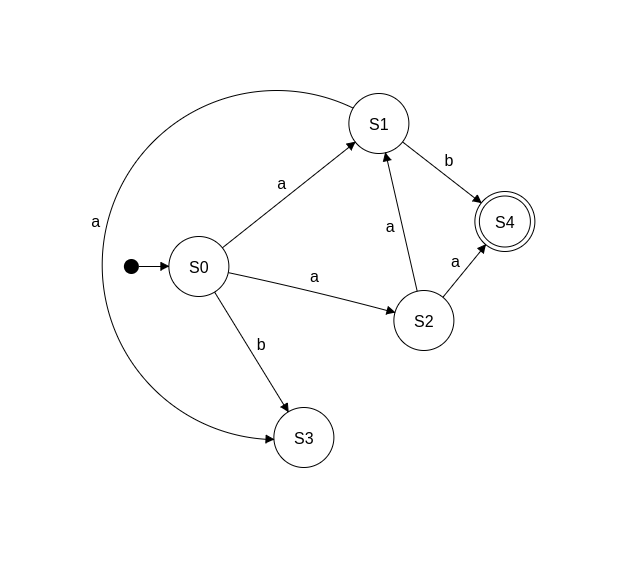
\includegraphics[width=1\textwidth]{fsm_schema.png}
    \caption{NFA FSM}
    \label{fig:example_image}
\end{figure}


As mentioned NFA's are primarily a useful theoretical abstraction. In hardware implementation of FSM's it is only possible to design DFA's and it is not possible to directly implement an NFA since logical circuits are sequential in nature. However, NFA's can be converted to DFA's. 

\subsection*{Acceptors}
An acceptor is an FSM that ends in an "accepted" or "non-accepted" final state, essentially the FSM finishes working in a final state which is valid or invalid. Each state of an acceptor is accepted or rejected, valid or invalid. Essentially if a state receives some input it either accepts the input or rejects it, the next state transition is dependent on whether it accepts or not. Acceptors can have multiple final states. Acceptors can be useful for pattern matching of strings sequences. Acceptors are used by, for example, Regex engines.

\subsection*{Classifiers}
Classifiers are a generalization of acceptors, classifiers have an output set greater than 2.

\subsection*{Transducers}

Transducers are FSM's whose output depends on the current state and / or input. 

\subsubsection*{Moore machines}
Moore machines are transducer FSM's whose output only depends on the current state. Moore machines are more easily comprehensible in the context of logical circuit design. An example of a moore machine logical circuit is shown below. 
\begin{figure}[H]
    \centering
    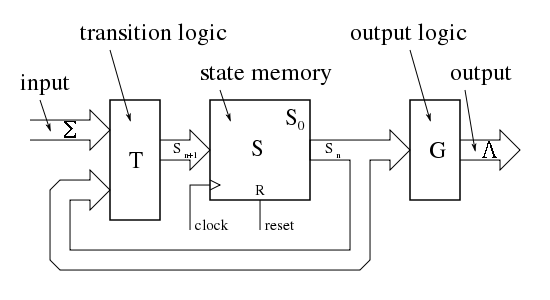
\includegraphics[width=1\textwidth]{moorecirc.png}
    \caption{An example of a moore circuit, picture taken from wikimedia commons}
    \label{fig:example_image}
\end{figure}

\subsubsection*{Mealy machines}
Mealy machines are transducers whose output depends on both the current state and the input. Similarly to Moore machines, Mealy machines are also the most easy to comprehend in the context of digital circuits.  I made a Mealy machine in Logisim to use an example of a Mealy machine.

\begin{figure}[H]
    \centering
    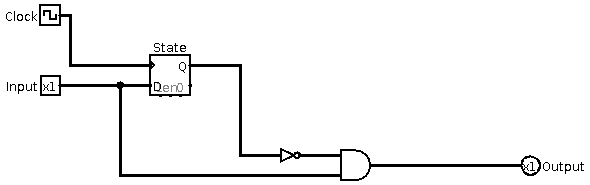
\includegraphics[width=1\textwidth]{mealymachine.png}
    \caption{An example of a Mealy circuit}
    \label{fig:example_image}
\end{figure}

The circuit is a simple pulse generator. It ensures that the incoming input that could last for
many clock cycles is output as a pulse that in the worst case lasts for just about one clock cycle. 


\section*{Designing FSM's step by step}
This is guide is primarily in the context of logical circuit design. 

\subsection*{Abstract state machine diagram}
The first step is to create an abstract state machine diagram. Allow states, inputs, outputs to have abstract descriptions. It is good to have an idea early on regarding the type of FSM you are aiming to design, is it an acceptor, transducer, etc. 

\subsection*{Encoding abstractions}
The second step is to encode the abstractions. I prefer to encode the abstractions in binary systems, but any number system should be sufficient. The most important thing is to encode inputs and outputs; state encoding can be omitted. 

\subsection*{State transition and output table}
In the final step, create a table with three columns, two if you have no output. The first column contains rows of current state's, The second column consists of subcolumns for each input. If the FSM is a Moore machine, there should be a third column with all the outputs associated with each state; if it is a mealy machine, there should be a sub-column for each input. 


\end{document}
